\chapter{Teori}

En stepper motor er en elektromotor der kan bevæges i små trin af en bestemt vinkel, ofte 1.8 eller 0.9 grader afhængig af motoren, dette giver en meget præcis positionering til forskel fra de mere gængse DC motorer der er bedre egnet til kontinuerte bevægelser der skal foregå flydende.

Steppermotorerne har flere fordele, i sammenhæng med WinePrep er de valgt da præcis positionering samt evnen til at gentage denne positionering er vigtig. Derudover har vi behov for en rigtig god evne til at bevare en given stillestående position på trods af ekstra belastninger, og her kommer stepper motorens rigtig gode hold torque til sin ret.

Stepper motorer kommer i flere varianter, og i WinePrep anvendes der både bipolare samt unipolare stepper motore. I dette dokument fokuseres der udelukkende på Bipolare stepper motore. Ønskes der information om brugen af unipolare stepper motore kan denne findes i dokumentet "Unipolære steppermotorer".

\section{Bipolar Stepper Motor}

Den bipolære steppermotor adskiller sig som det ses på figur \ref{bipolarlayout} fra den unipolære stepper motor ved at have 1 vikling per fase hvor den unipolære har 1 fælles tab i midten af spolen.

Afhængig af polariteten i den givne spole vil motoren rotere sin akse til den givne position.

\begin{figure}[H]
	\centering
	\caption{Biporlar stepper motors konstruktion}
	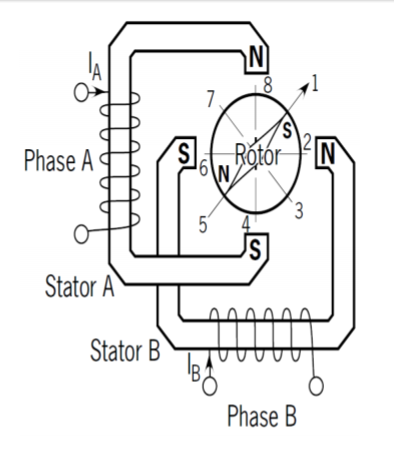
\includegraphics{billeder/konstruktion}
	\label{bipolarlayout}
\end{figure}

Til WinePrep anvedes der kun stepper motorer med gearing, hvilket gør at vi ikke anvender microstepping, da vi allerede uden dette har en rigelig god præcision.

For at anvende en bipolar stepper til full step skal faserne påtrykkes spænding ud fra lookup tabellen på figur \ref{lookuptabel}.

\begin{figure}[H]
	\centering
	\caption{lookup tabel for bipolar stepper motor}
	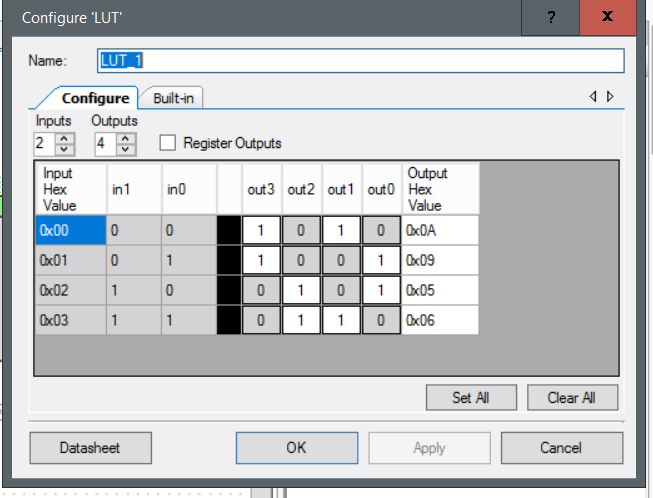
\includegraphics{billeder/lookup}
	\label{lookuptabel}
\end{figure}

Den bipolare stepper motor styres med 1 fuld h-bro pr fase. 